\documentclass[11pt]{beamer}
\usetheme{OIE}
\usepackage[utf8]{inputenc}
\usepackage[german]{babel}
\usepackage[T1]{fontenc}
\usepackage{amsmath}
\usepackage{amsfonts}
\usepackage{amssymb}
\usepackage{tikz}
\usepackage{graphicx}
\usepackage{color}
\usepackage{booktabs}
\usepackage{pifont}
\usepackage{xcolor}
\usepackage[natbib=true,backend=bibtex,style=authoryear]{biblatex}
\author{Dominik Both, Tonio Weidler}
\title{Open Information Extraction}
%\setbeamercovered{transparent} 
%\setbeamertemplate{navigation symbols}{} 
%\logo{} 
\institute{Institut für Computerlinguistik, Universität Heidelberg} 
\date{15.07.2016} 
\subject{} 
\definecolor{lightgray}{gray}{0.8}

\begin{document}

% AUTOMATISMEN
\AtBeginSection{\frame{\sectionpage}}
\AtBeginSubsection{\frame{\subsectionpage}}


% TEMPLATING
\setbeamertemplate{title page}{
	\center 
		\begin{beamercolorbox}[center]{part title}
	      \Huge\inserttitle\par
	    \end{beamercolorbox}
	    \vspace{15pt}
		\insertauthor\\
		\vspace{15pt}		
		Proseminar \textit{Text Mining}\\
		Andrea Zielinski\\
		\vspace{15pt}
		\insertinstitute, \insertdate
}

\defbeamertemplate{section page}{wiqe}[1][]{%
  \begin{centering}
    \begin{beamercolorbox}[center]{part title}
      \Huge\insertsection\par
    \end{beamercolorbox}
  \end{centering}
}

\defbeamertemplate{subsection page}{wiqe}[1][]{%
  \begin{centering}
    \begin{beamercolorbox}[center]{}
      \usebeamerfont{subsection title}\usebeamercolor[fg]{subsection name}\insertsection\par
    \end{beamercolorbox}
    \begin{beamercolorbox}[sep=2pt,center]{part title}
		\huge\insertsubsection\par
    \end{beamercolorbox}
  \end{centering}
}
\setcounter{tocdepth}{1}
\setbeamertemplate{section page}[wiqe]
\setbeamertemplate{subsection page}[wiqe]

% COMMANDS
\newcommand{\hitem}{
	\item[\color{lightgray}\rule{0.5em}{0.5em}]
}

\begin{frame}
\titlepage
\end{frame}

\begin{frame}{Strukturierung}
    \tableofcontents
\end{frame}

\section{Introduction to Information Extraction}
	\begin{frame}{What is Information Extraction?}
			\begin{center}
				Goal of Information Extraction is automatically extracting information from unseen text
				Information: entities, relations, events...
				
				To make the dough for a good pizza, we start with putting 1kg of flour into the mixing bowl.
				(1kg of flour, put into, mixing bowl)
			\end{center}
	\end{frame}
	\begin{frame}{Problems of Information Extraction}
				\begin{center}
				\begin{itemize}
					\item Named Entity Recognition
					\item Relationship Extraction 
					\item Coreference Resolution
					\item Comment Extraction
					\item many more
					\end{itemize}
				\end{center}
	\end{frame}
\section{OIE - Principles}
	\subsection{Open Information Extraction}
		\begin{frame}{Open Information Extraction}
			\begin{center}
				\begin{itemize}
				IE: Extractor for each target relation
				Open: No pre-specified extractors
					Unsupervised learning of relation phrases
				Extraction of information on every given domain
				\end{itemize}
			\end{center}
		\end{frame}
		\begin{frame}{Problems of Open Information Extraction}
					\begin{center}
						\begin{itemize}
						\item Incoherent extractions:
							\item This guide contains dead links and omits sites -> contains omits
						\item Uninformative extractions:
							\item Faust made a deal with the devil -> (Faust, made, a deal)
							\end{itemize}
					\end{center}
				\end{frame}
	\subsection{Methods}
		\begin{frame}{Text Runner and WOE}
			\begin{center}
				\begin{itemize}
				\item 1. Label: Automatic sentence labeling by heuristics
				\item 2. Learn: A relation phrase extractor is learned
				\item 3. Extract: Identifying NP pairs and searching relations words between
				\end{itemize}
			\end{center}
		\end{frame}
		\begin{frame}{Problems}
					\begin{center}
						\begin{itemize}
						\item Large number of labeled training examples required
						\item Alternative heuristic labeling leads to huge noise and stacked uncertainty
						\item Ignores both holistic and lexical aspects 
						\end{itemize}
					\end{center}
				\end{frame}
		
		
		\begin{frame}{Syntactic constraint}
			\begin{center}
				\begin{itemize}
				\item Limits relations to those matching a certain POS Tag pattern:
				\item V | V P | VW* P %ich mache dann Beispiele was das heißt
				\item Always choses longest possible match
				\item Merge ajacent matches together
				\end{itemize}
				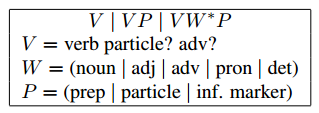
\includegraphics[scale=0.5]{img/pos.png}\\
				%beispiel mit faust
			\end{center}
		\end{frame}
		\begin{frame}{Lexical constraint}
			\begin{center}
				\begin{itemize}
				\item Only assume relations that appear in the corpus for a certain amount
				\item The Obama administration \textbf{is offering only modest greenhouse gas reduction targets at} the conference
				\end{itemize}
			\end{center}
		\end{frame}
		\begin{frame}{Limitations of those constraints}
			\begin{center}
				\begin{itemize}
				\item In a set of 300 hand-annotated sentences 85\% relations fell into those constraints
				\item Model is not complete and has its flaws
				\end{itemize}
				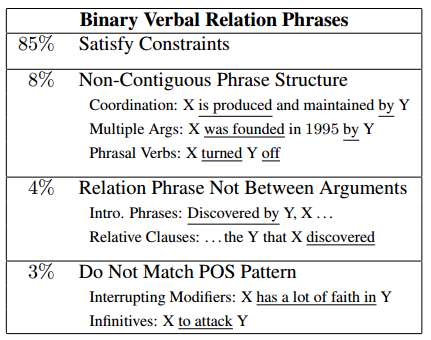
\includegraphics[scale=0.5]{img/constraints.png}\\	
			\end{center}
		\end{frame}
		\begin{frame}{ReVerb Extraction Algorithm}
			\begin{center}
				\begin{itemize}
				\item Relation Extraction: Find the longest possible string of words that match the relation constraints, merge adjacents
				\item Argument Extraction: Find the nearest NP left and right to the relation that is not a relativ pronoun, WHO-adverb or existential-there.
				\item How is the lexical constraint being checked? By creating a list of relational phrases by applying this algorithm on a 500 million Web sentences.
				\end{itemize}
			\end{center}
		\end{frame}
		\begin{frame}{ReVerb Confidence Function}
					\begin{center}
						\begin{itemize}
						\item The Algorithm has a high recall, but low precision
						\item Now the extracted relation is weighted by a confidence function:
						\end{itemize}
						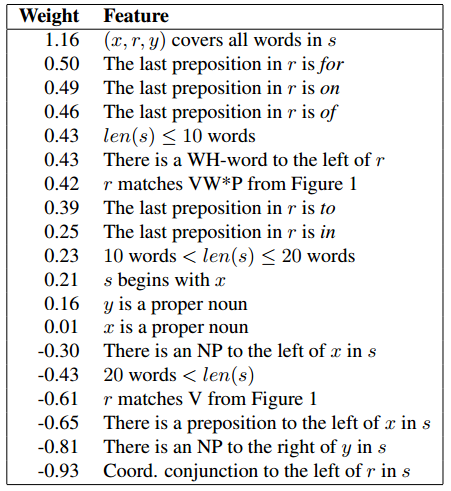
\includegraphics[scale=0.5]{img/sososo.png}\\
					\end{center}
				\end{frame}
	\subsection{Data Representation}
		\begin{frame}{Standard Patterns}
			\begin{center}
				\includegraphics[scale=0.5]{img/oie-pattern.png}\\
				\vspace{15pt}
				\textbf{Argument A} is in a directed \textbf{relation} to \textbf{Argument B}.
			\end{center}
		\end{frame}
		
		\begin{frame}{Unnormalized Annotation}
			\begin{center}
				(argument\_a, predicate\_x, argument\_b)\\
				(argument\_a, predicate\_y, argument\_c)\\
				(argument\_a, predicate\_y, argument\_d)
			\end{center}
			\vspace{15pt}
			\textbf{Problems}\\
			\begin{itemize}
				\item redundant
				\item unnormalized
				\item can only produce binary predicates
			\end{itemize}
		\end{frame}
		
		\begin{frame}{RDF and Linked Data}
			\begin{block}{Resource Description Framework}
				Models propositions by constructing \textit{triples} including \textbf{Subjects}, \textbf{Objects} and \textbf{Predicates}\\
				Generates a directed graph
			\end{block}
			\vspace{10pt}
			\begin{center}
				:subject :predicate :object.
				\vspace{10pt}
				\includegraphics[scale=0.5]{img/oie-rdf-triple.png}
			\end{center}
		\end{frame}
		
		\begin{frame}{RDF Concepts and Notation}
			\begin{itemize}
				\item \textbf{URIs}\\
					identifies ressources (S, R, O) distinctivly and references further informations (triples)
				\item \textbf{Conclusions}\\
					allows to draw conclusions using rules
				\item \textbf{Turtle}\\
					allows syntax abbreviations
			\end{itemize}
		\end{frame}
		
		\begin{frame}[fragile]{RDF Syntax}
			\begin{verbatim}
				dbr:Barack_Obama a foaf:person, :President;
				    dbo:spouse dbr:Michelle_Obama.
				dbr:Bernie_Sanders dbo:birthPlace dbr:New_York, 
				                                  dbr:Brooklyn;
				dbr:Brooklyn dbo:isPartOf dbr:New_York 	
			\end{verbatim}
		\end{frame}
		
		\begin{frame}{... als Graph}
			\begin{center}
				\includegraphics[scale=0.4]{img/oie-rdf-example.png}
			\end{center}			
		\end{frame}
\section{Example: LODifier}
	\subsection{Architecture}
	\subsection{Preprocessing}
	\subsection{RDF Construction}
	\subsection{Conclusions}
\section{OIE Systems in Context}
	\subsection{Comparison}
	\subsection{Evaluating the Approaches}
\section{Conclusion}
	\subsection{Problems and Obstacles}
	\subsection{Future Opportunities}

\end{document}